%label:"art:applicationsOfSH"
%author:JeffHicks
%name:"applications of $\SH(X)$"
%type:"article"

We look at some applications and theorems from symplectic cohomology. 
%tag:000T
%label:prp:homologyIncludesIntoSH
%author:JeffHicks
%name:"cohomology includes into SH"
%type:proposition

 
 \label{prp:homologyIncludesIntoSH}
Let $X$ be a Liouville domain. There is a map 
\[H^\bullet(X)\to \SH(X).\]
 
%label:"prf:homologyIncludesIntoSH"
%parent:"prp:homologyIncludesIntoSH"
%author:JeffHicks
%name:"cohomology includes into SH"
%type:"proof"

 
    Let $m_0$ be the minimal period of a Reeb orbit in $(\partial X, \alpha)$. Pick a slope $0< m< m_0$, and consider a linear Hamiltonian $H^m$ which is $C^2$ small on $X$. Then the only orbits for $H^m$ will be the constant orbits, and there is a quasi-isomorphism of chain complexes between $\CF(\hat X, H^m_t)$ and the Morse complex $CM^\bullet(\hat X, H^m_t)$ sending each constant orbit to its associated critical point of $H^m_t$. Since $H^m$ has gradient which points outward along the boundary of $X$, this is a valid Morse function for computing the Morse cohomology of $X$.
 
%author:JeffHicks
%name:"Weinstein conjecture for hypersurfaces in $\RR^n$"
%type:"application"
%label:"app:weinsteinConjectureInRn"
%parent:"prp_homologyIncludesIntoSH"

\begin{application}
We look at an application of \cref{prp:homologyIncludesIntoSH}. 
Let $X$ be a Liouville domain, and suppose that $(\partial X, \alpha)$ has no Reeb orbits. Then the map from \cref{prp:homologyIncludesIntoSH} is an isomorphism 
\[H^\bullet(X)\to \SH(X).\]
Therefore, we can compute $\SH(X)$ to show that $(\partial X)$ has a Reeb orbit.  

%label:"exm:SHofBall"
%name:"symplectic cohomology of the ball"
%type:"example"

A key example is the standard contact structure on the sphere. One can compute that the standard symplectic ball $B^{2n}:=\{(z_1, \ldots, z_n)\st \sum_{i=1}^n |z_i|^2=1 \}\subset \CC^n$ is a Liouville domain, and that $\SH(B^{2n})=0$. We can conclude that $(S^{2n-1}, \alpha)$ has a Reeb orbit.

A generalization of this result (due to \cite{oancea2003suite}) states that whenever $X$ is a subcritical  \snip{Stein domain}{exm:steinDomain} (so the Morse indexes of the critical points of $\phi: X\to \RR$ are all less than $n$) then $\SH(X)=0$. 
\end{application}
%label:"def:liouvilleSubomain"
%author:JeffHicks
%name:"Liouville subdomain"
%type:"definition"

 
    Suppose that $(X, \lambda)$ is a Liouville domain. A \emph{Liouville subdomain} is a compact submanifold with boundary $X_0\subset X\setminus \partial X$ such that the Liouville vector $Z$ points outwards along $\partial X_0$.
 \label{def:liouvillesubDomain}
 
%label:thm:viterboRestriction
%author:JeffHicks
%name:"Viterbo restriction"
%type:theorem
%source:viterbo1999functors


    \label{thm:viterboRestriction}
    Let $X_0\subset X$ be a Liouville subdomain. Then there is a restriction map $\SH(X)\to \SH(X_0)$, which is a unital ring homomorphism. Furthermore, we have a commutative diagram
    %tag:000X
%label:"dig:viterboSuggestive"
%type:"diagram"
%parent:thm:viterboRestriction
%author:JeffHicks

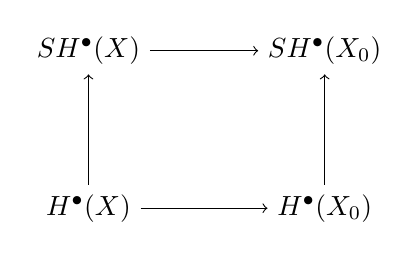
\begin{tikzpicture}

    \node (v3) at (-2,1) {$SH^\bullet(X)$};
    \node (v4) at (1,1) {$SH^\bullet(X_0)$};
    \node (v1) at (-2,-1) {$H^\bullet(X)$};
    \node (v2) at (1,-1) {$H^\bullet(X_0)$};
    \draw  (v1) edge[->] (v2);
    \draw  (v1) edge[->] (v3);
    \draw  (v3) edge[->] (v4);
    \draw  (v2) edge[->] (v4);
\end{tikzpicture}
    where the horizontal maps are given by \cref{prp:homologyIncludesIntoSH}.

In the setting of subcritical Stein domains ( 
\cref{app:weinsteinConjectureInRn} ), the sublevel sets $X|_{\phi< t}$ 
form 
a nested sequence of Liouville subdomains. One way to prove the vanishing of $\SH(X)$ is to show that the map $\SH(X|_{\phi< t_{i+1}})\to \SH(X|_{\phi< t_{i}})$ is a an isomorphism for all $t_{i} < t_{i+1}$. When the only critical points of $\phi$ contained in $\SH(X|_{\phi < t_0})$ are minima, then $X|_{t_0}$ is a ball, which has vanishing symplectic cohomology.
